%!TEX root=../../autopilot.tex
\section{Sound Latency}
\label{sec:soundlatency}

We measured end to end, hardware input to hardware output latency by measuring the delay between a digital input and the onset of a 10kHz pure tone (Table \ref{tab:materials}). 

Autopilot's \href{http://jackaudio.org/}{jack} audio backend was configured with a \texttt{192kHz} sampling rate and a total buffer size of \texttt{128} samples, for theoretical minimum latency of \texttt{0.67ms}\sidenote{A previous version of this paper included benchmarking and comparison to Bpod and pyControl's sound onset latency, but since then both packages have changed substantially, including Bpod creating a new \href{https://sites.google.com/site/bpoddocumentation/assembling-bpod/hifi-module}{hifi sound module} based off very similar HiFiBerry hardware that we use here, making those benchmarks obsolete. We have omitted similar comparative benchmarks here in favor of allowing the maintainers of those packages to publish their own due to the cost of acquiring the new hardware, the version dependency of any benchmarks, and the distraction from characterizing the system at hand.}.

For both systems we directly measured the input logic and output sound voltage with an oscilloscope and estimated latency with its measurement cursors. %
%
\begin{figure}[hb!]
\caption{For the two systems we measured (blue), mean latency is presented $\pm$ standard deviation of all individual measurements (black dots, n=200 for each). Reported latencies (red) of \href{https://sites.google.com/site/bpoddocumentation/bpod-user-guide/function-reference/psychtoolboxsoundserver}{Bpod} and \href{https://pycontrol.readthedocs.io/en/latest/user-guide/hardware/\#audio_player}{pyControl} were found online.}
\label{fig:lags}
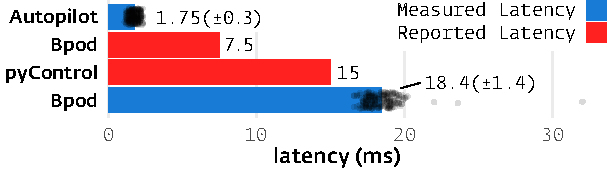
\includegraphics{figures/test_1_lags.pdf}
\end{figure}

Autopilot's  \texttt{1.75ms} $\pm$ \texttt{0.3} latency---less than 3x the theoretical minimum---improves upon the measured latency of Bpod and reported latency of pyControl by an order of magnitude (Figure \ref{fig:lags}, \texttt{18.4ms} $\pm$ \texttt{1.4}, \texttt{15ms} respectively). This suggests that Autopilot eliminates most perceptible end-to-end latency, which is necessary for tasks that require realtime feedback. One clear future direction is to write the sound processing loop in a compiled language exposed with a foreign function interface (FFI) to improve its performance.